\documentclass{article}
\usepackage{listings}
\usepackage[T1]{fontenc}
\usepackage{beramono}
\usepackage[usenames,dvipsnames]{xcolor}
\usepackage{color}
\usepackage{fancyhdr}
\usepackage{extramarks}
\usepackage{amsmath}
\usepackage{amsthm}
\usepackage{amsfonts}
\usepackage{tikz}
\usepackage{bold-extra}
\usepackage[plain]{algorithm}
\usepackage{algpseudocode}
\usepackage{pdfpages}
\usepackage{soul}
\usepackage[
    backend=biber,
    doi=false,
    url=false,
    eprint=false,
    isbn=false,
]{biblatex}
\addbibresource{misc/ref.bib}
\usetikzlibrary{automata,positioning}

\definecolor{mygreen}{RGB}{28,172,0} % color values Red, Green, Blue
\definecolor{mylilas}{RGB}{170,55,241}
\definecolor{backcolour}{rgb}{0.95,0.95,0.92}
%
% Basic Document Settings
%

\topmargin=-0.45in
\evensidemargin=0in
\oddsidemargin=0in
\textwidth=6.5in
\textheight=9.0in
\headsep=0.25in

\linespread{1.1}

\pagestyle{fancy}
\lhead{\noteAuthorName}
\rhead{\leftmark}
\lfoot{\lastxmark}
\cfoot{\thepage}

\renewcommand\headrulewidth{0.4pt}
\renewcommand\footrulewidth{0.4pt}
\renewcommand{\baselinestretch}{1.5}

\setlength\parindent{0pt}

\setcounter{secnumdepth}{0}

\newcommand{\noteTitle}{Homework \#4}
\newcommand{\noteAuthorName}{\textbf{Daniel Deng}}

%
% Title Page
%

\title{
    \vspace{2in}
    \textmd{\textbf{\noteTitle}}\\
    \vspace{3in}
}

\author{\noteAuthorName}
\date\today

\renewcommand{\part}[1]{\textbf{\large Part \Alph{partCounter}}\stepcounter{partCounter}\\}

%
% Various Helper Commands
%

% Useful for algorithms
\newcommand{\alg}[1]{\textsc{\bfseries \footnotesize #1}}

% For derivatives
\newcommand{\deriv}[1]{\frac{\mathrm{d}}{\mathrm{d}x} (#1)}

% For partial derivatives
\newcommand{\pderiv}[2]{\frac{\partial}{\partial #1} (#2)}

% Integral dx
\newcommand{\dx}{\mathrm{d}x}

% Alias for the Solution section header
\newcommand{\solution}{\textbf{\large Solution}}

% Probability commands: Expectation, Variance, Covariance, Bias
\newcommand{\E}{\mathrm{E}}
\newcommand{\Var}{\mathrm{Var}}
\newcommand{\Cov}{\mathrm{Cov}}
\newcommand{\Bias}{\mathrm{Bias}}

% % Julia language
% \lstdefinelanguage{Julia}%
%   {morekeywords={abstract,break,case,catch,const,continue,do,else,elseif,%
%       end,export,false,for,function,immutable,import,importall,if,in,%
%       macro,module,otherwise,quote,return,switch,true,try,type,typealias,%
%       using,while,@test},%
%    sensitive=true,%
%    alsoother={$},%
%    morecomment=[l]\#,%
%    morecomment=[n]{\#=}{=\#},%
%    morestring=[s]{"}{"},%
%    morestring=[m]{'}{'},%
% }[keywords,comments,strings]%

% \definecolor{backcolour}{rgb}{0.95,0.95,0.92}

% \lstset{%
%     language         = Julia,
%     basicstyle       = \ttfamily,
%     keywordstyle     = \bfseries\color{blue},
%     stringstyle      = \color{magenta},
%     commentstyle     = \color{ForestGreen},
%     showstringspaces = false,
%     backgroundcolor = \color{backcolour},
%     inputencoding = utf8,
%     extendedchars = true,
%     breaklines      =   true,
%     literate=%
%                 {≈}{{$\approx$}}1
%                 {π}{{$\pi$}}1
%                 {∇}{{$\nabla$}}1
% }

%% matlab language
\lstset{language=Matlab,%
    %basicstyle=\color{red},
    backgroundcolor = \color{backcolour},
    breaklines=true,%
    morekeywords={matlab2tikz},
    keywordstyle=\color{blue},%
    morekeywords=[2]{1}, keywordstyle=[2]{\color{black}},
    identifierstyle=\color{black},%
    stringstyle=\color{mylilas},
    commentstyle=\color{mygreen},%
    showstringspaces=false,%without this there will be a symbol in the places where there is a space
    numbers=left,%
    numberstyle={\tiny \color{black}},% size of the numbers
    numbersep=9pt, % this defines how far the numbers are from the text
    emph=[1]{for,end,break},emphstyle=[1]\color{red}, %some words to emphasise
    %emph=[2]{word1,word2}, emphstyle=[2]{style},    
}


\begin{document}



    \maketitle
    \pagebreak
    % \tableofcontents
    % \pagebreak
    \section{Problem 1}
    State space representation from differential equations.

    \subsection{a)} 
    $2\ddot{x} + 4\dot{x} + 4x=3u$, where the state vector is 
    $\begin{bmatrix}
        x \\
        \dot{x}
    \end{bmatrix}$.
    The out put is x.
    \subsubsection{\textit{ Sol. }}
    $\ddot{x} + 2\dot{x} + 2x=1.5u$ $\Rightarrow$ 
    $\left\{
        \begin{array}{lr}
        \dot{x} = 0x + \dot{x} \\
        \ddot{x} = -2x -2\dot{x} + 1.5u
        \end{array}
    \right.$, thus

    \begin{align}
        \dot{\textbf{x}} &=
        \begin{bmatrix}
            \dot{x} \\
            \ddot{x}
        \end{bmatrix} = 
        \begin{bmatrix}
            0 & 1 \\
            -2 & -2
        \end{bmatrix}
        \begin{bmatrix}
            x \\
            \dot{x}
        \end{bmatrix} + 
        \begin{bmatrix}
            0\\
            1.5
        \end{bmatrix}
        u
        \\
        y&=
        \begin{bmatrix}
            x
        \end{bmatrix} =
        \begin{bmatrix}
            1 & 0
        \end{bmatrix}
        \begin{bmatrix}
            x \\
            \dot{x}
        \end{bmatrix} + 
        \begin{bmatrix}
            0
        \end{bmatrix}
        u
    \end{align}

    We get:

    \begin{equation}
        \textbf{A} =
        \begin{bmatrix}
            0 & 1 \\
            -2 & -2
        \end{bmatrix}, 
        \textbf{B} =
        \begin{bmatrix}
            0\\
            1.5
        \end{bmatrix}, 
        \textbf{C} =
        \begin{bmatrix}
            1 & 0
        \end{bmatrix}, 
        \textbf{D} =
        \begin{bmatrix}
            0
        \end{bmatrix}
    \end{equation}

    \subsection{b)} 
    $2\ddot{x} + 4\dot{x} + 4x=3u$, where the state vector is 
    $\begin{bmatrix}
        x + \dot{x} \\
        \dot{x}
    \end{bmatrix}$.
    The out put is x.

    \subsubsection{\textit{ Sol. }}
    $\left\{
        \begin{array}{lr}
        \dot{x} + \ddot{x} = \dot{x} + (-2x -2\dot{x} + 1.5u) = -2(x + \dot{x}) + \dot{x} + 1.5u\\
        \ddot{x} = -2x -2\dot{x} + 1.5u = -2(x + \dot{x}) + 0\dot{x} + 1.5u \\
        x = (x + \dot{x}) + (-1)\dot{x}
        \end{array}
    \right.$, thus

    \begin{align}
        \dot{\textbf{x}} &=
        \begin{bmatrix}
            \dot{x} + \ddot{x}\\
            \ddot{x}
        \end{bmatrix} = 
        \begin{bmatrix}
            -2 & 1 \\
            -2 & 0
        \end{bmatrix}
        \begin{bmatrix}
            x + \dot{x}\\
            \dot{x}
        \end{bmatrix} + 
        \begin{bmatrix}
            1.5\\
            1.5
        \end{bmatrix}
        u
        \\
        y&=
        \begin{bmatrix}
            x
        \end{bmatrix} =
        \begin{bmatrix}
            1 & -1
        \end{bmatrix}
        \begin{bmatrix}
            x + \dot{x}\\
            \dot{x}
        \end{bmatrix} + 
        \begin{bmatrix}
            0
        \end{bmatrix}
        u
    \end{align}

    We get:

    \begin{equation}
        \textbf{A} =
        \begin{bmatrix}
            -2 & 1 \\
            -2 & 0
        \end{bmatrix}, 
        \textbf{B} =
        \begin{bmatrix}
            1.5\\
            1.5
        \end{bmatrix}, 
        \textbf{C} =
        \begin{bmatrix}
            1 & -1
        \end{bmatrix}, 
        \textbf{D} =
        \begin{bmatrix}
            0
        \end{bmatrix}
    \end{equation}
    

    \subsection{c)}
    Using the A,B,C,D matrices found in parts (a) and (b), use Matlab's step command to simulate the step responses to both systems. How do these step responses compare and does that comparison make sense? 
    \subsubsection{\textit{ Sol. }}
    Matlab code:
    \lstinputlisting{codes/Question1c.m}
    Result:
    \begin{figure}[htp]
        \centering
        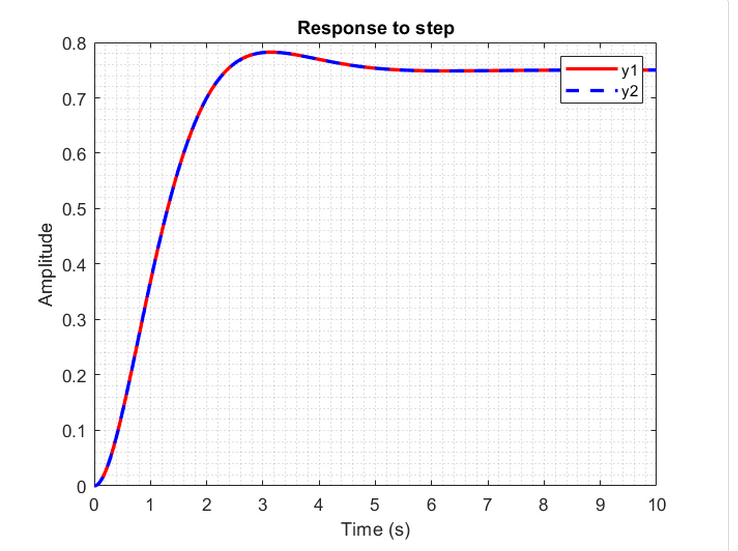
\includegraphics[width=15cm]{images/Q1_c_fig.png}
        \caption{Step Response}
        \label{fig:Q1c}
    \end{figure}

    We can tell from Fig.\ref{fig:Q1c} that the step responses are exactly the same.
    This make sense because we are representing the same system, and the output is the same for the two representations. 

\pagebreak
    \section{Problem 2}
State space representation of a 2-mass system.

For the following mechanical system, there is one input, $f$, and two outputs: the position of the first mass, $z_1$, and the distance between the masses, $z_1 - z_2$.

\begin{figure}[htp]
    \centering
    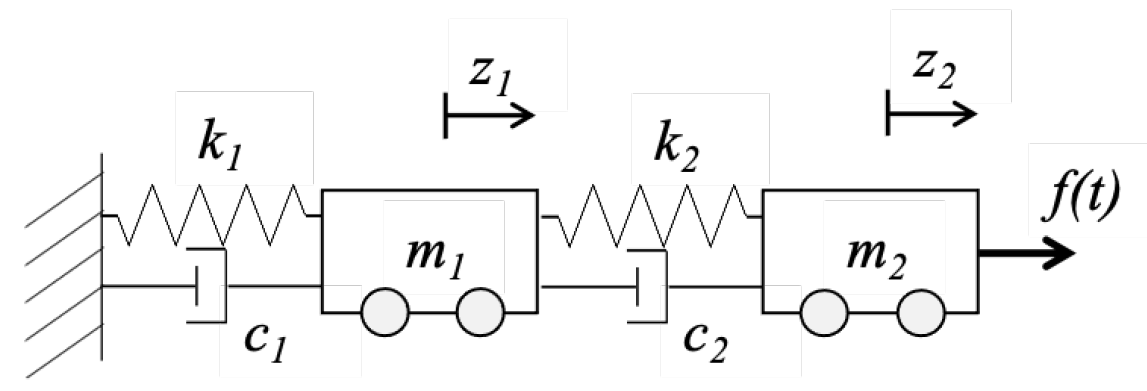
\includegraphics[width=15cm]{images/Q2.png}
\end{figure}

\subsection{a)}
Write the state equation, $\dot{x}=Ax+Bu$, where $x$ is a state vector that you choose, $A$ is the system matrix, $B$ is the input matrix, and $u$ is the input.
\subsubsection{\textit{ Sol. }}

First we identify all energy storage elements:

\begin{table}[ht]
    \centering
    \begin{tabular}{c | c}
        Energy Storage Elements & State variable
        \\
        \hline
        $m_1$ (Kinetic) & $\dot{z_1}$ \\
        $m_2$ (Kinetic) & $\dot{z_2}$ \\
        $k_1$ (Potential) & $z_1$ \\
        $k_2$ (Potential) & $z_2 - z_1$
    \end{tabular}
\end{table}

From all energy storage elements we define the state vector: $\textbf{x} = 
\begin{bmatrix}
    x_1\\
    x_2\\ 
    x_3\\ 
    x_4
\end{bmatrix} = 
\begin{bmatrix}
    z_1\\
    z_2 - z_1\\ 
    \dot{z_1}\\ 
    \dot{z_2}
\end{bmatrix}$, and input $u = f$

Draw FBD to analyze system dynamics: 
\begin{figure}[htp]
    \centering
    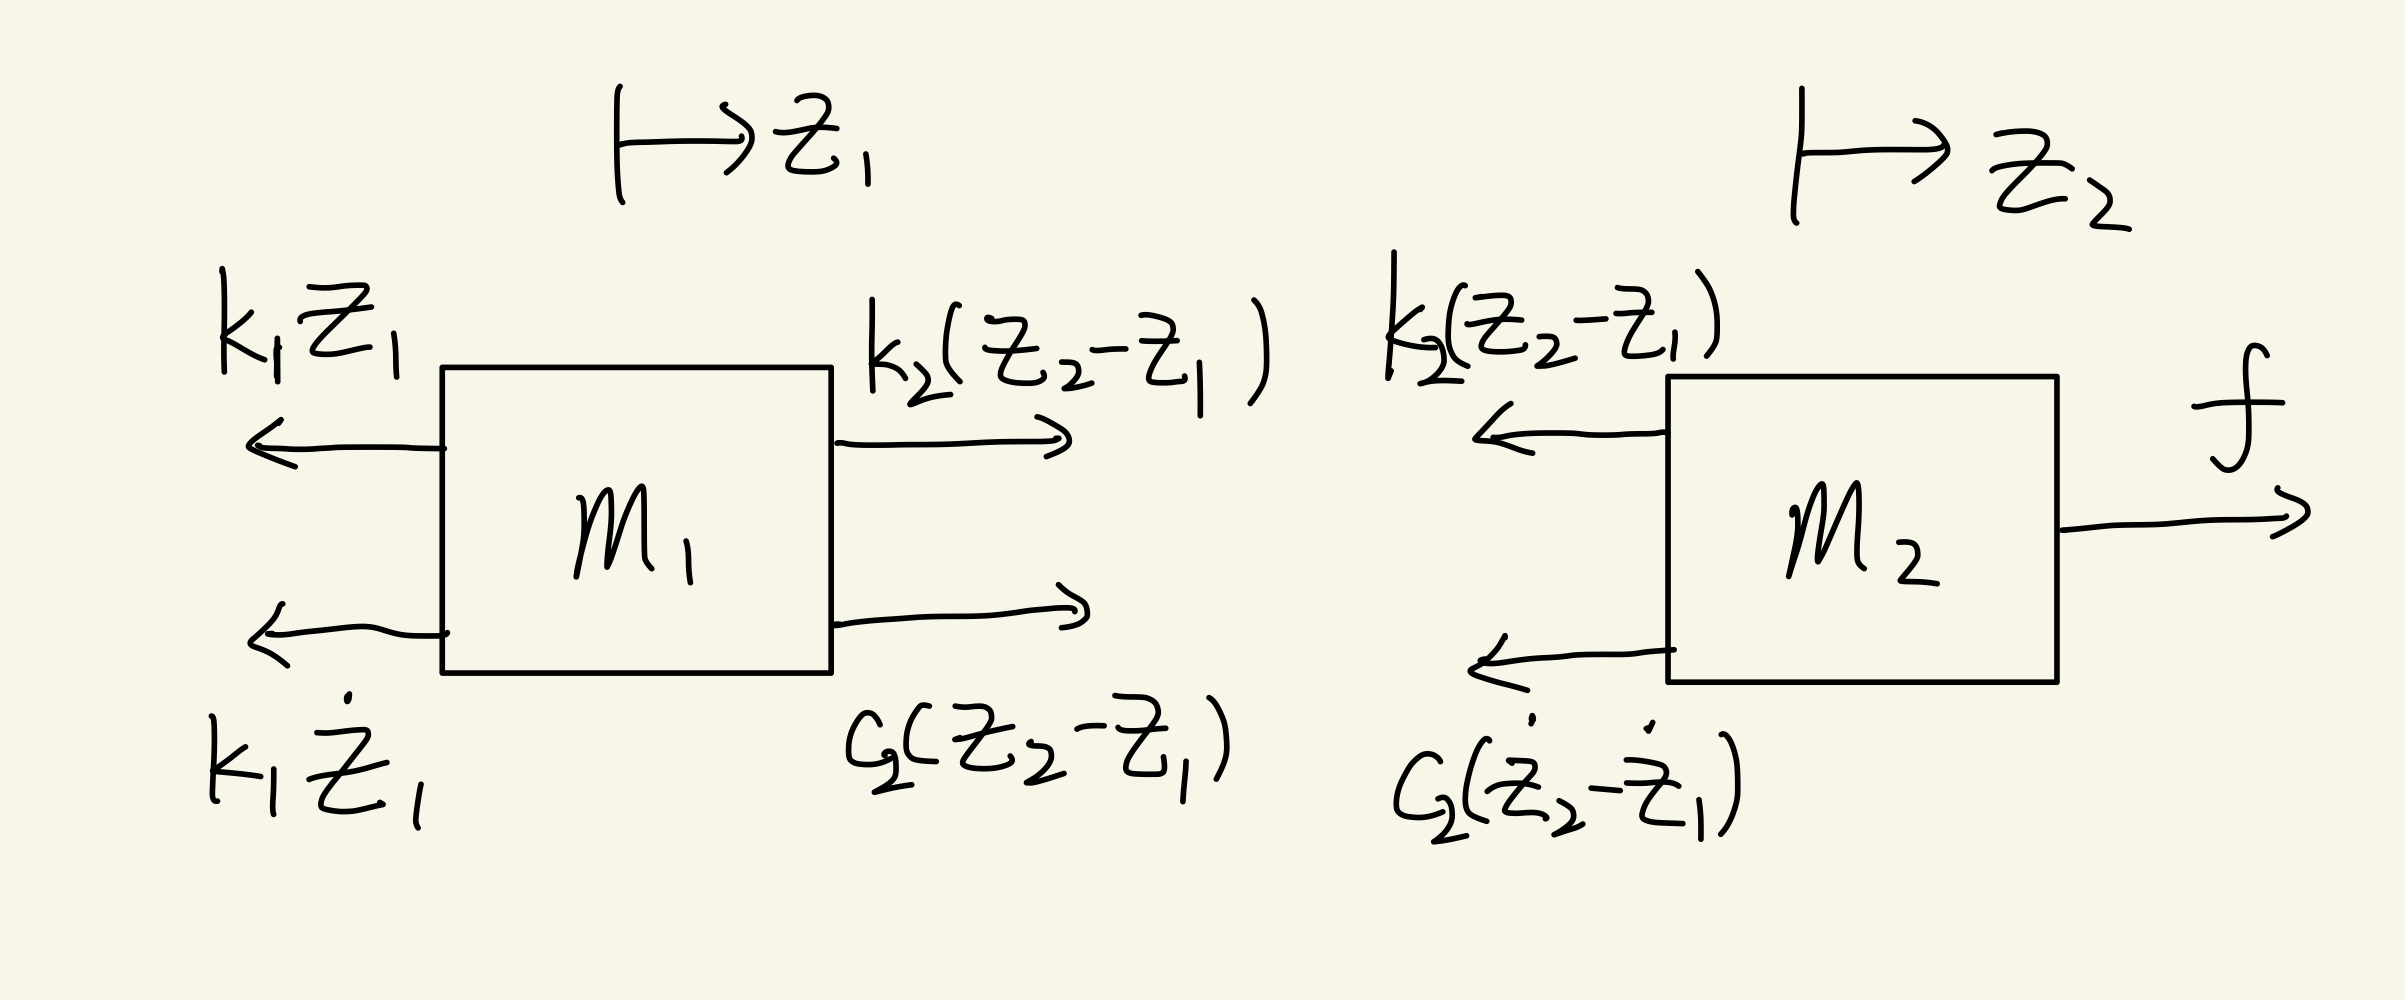
\includegraphics[width=10cm]{images/Q2_FBD.png}
    \caption{Free body diagram}
    \label{fig:Q2FBD}
\end{figure}

We get the following dynamic equations:

$\left\{
    \begin{array}{lr}
    m_1\ddot{z_1} = k_2(z_2 - z_1) + c_2(\dot{z_2} - \dot{z_1}) - k_1z_1 -c_1\dot{z_1}\\
    m_2\ddot{z_2} = f - k_2(z_2 - z_1) - c_2(\dot{z_2} - \dot{z_1})\\
    \end{array}
\right.$ 

$\Rightarrow $
$\left\{
    \begin{array}{lr}
    \dot{x_1} = \dot{z_1} \\ 
    \dot{x_2} = \dot{z_2} - \dot{z_1}\\
    \dot{x_3} = \ddot{z_1} = \frac{k_2}{m_1} (z_2 - z_1) + \frac{c_2}{m_1}(\dot{z_2} - \dot{z_1}) - \frac{k_1}{m_1}z_1 -\frac{c_1}{m_1}\dot{z_1}\\
    \dot{x_4} = \ddot{z_2} = \frac{f}{m_2} - \frac{k_2}{m_2}(z_2 - z_1) - \frac{c_2}{m_2}(\dot{z_2} - \dot{z_1})\\
    \end{array}
\right.$

$\Rightarrow $
$\left\{
    \begin{array}{lr}
    \dot{x_1} = 0x_1 + 0x_2 + x_3 + 0x_4 + 0u \\ 
    \dot{x_2} = 0x_1 + 0x_2 + (-1)x_3 + x_4 + 0u \\
    \dot{x_3} = - \frac{k_1}{m_1}x_1 + \frac{k_2}{m_1} x_2 - \frac{c_1+c_2}{m_1}x_3 + \frac{c_2}{m_1}x_4 + 0u\\
    \dot{x_4} = 0x_1 - \frac{k_2}{m_2}x_2 + \frac{c_2}{m_2}x_3 - \frac{c_2}{m_2}x_4 + \frac{1}{m_2}u\\
    \end{array}
\right.$

We can write the state space equation as:
\begin{equation}
    \dot{\textbf{x}} =
        \begin{bmatrix}
        0                & 0                & 1                    & 0 \\
        0                & 0                & -1                   & 1 \\ 
        -\frac{k_1}{m_1} & \frac{k_2}{m_1}  & -\frac{c_1+c_2}{m_1} & \frac{c_2}{m_1}  \\ 
        0                & -\frac{k_2}{m_2} & \frac{c_2}{m_2}      & -\frac{c_2}{m_2}
    \end{bmatrix}
    \textbf{x} + 
    \begin{bmatrix}
        0\\
        0\\ 
        0\\ 
        \frac{1}{m_2}
    \end{bmatrix}
    u
\end{equation}

\subsection{b)}
Write the output equation, $y = Cx + Du$.
\subsubsection{\textit{ Sol. }}
The output vector: $\textbf{y} = 
\begin{bmatrix}
    z_1\\
    z_1 - z_2
\end{bmatrix} = 
\begin{bmatrix}
    x_1\\
    - x_2
\end{bmatrix}$, thus: 

\begin{equation}
    \textbf{y} =
        \begin{bmatrix}
        1 & 0  & 0 & 0 \\
        0 & -1 & 0 & 0 \\ 
    \end{bmatrix}
    \textbf{x} + 
    \begin{bmatrix}
        0\\
        0
    \end{bmatrix}
    u
\end{equation}

\pagebreak
    \section{Problem 3}
Changing the system matrix with state feedback.

The rotary mass-spring-damper system shown below has an input torque $u = T$ and
output position $\theta$ with a rotational spring $k_{\theta}$ and rotational damper $c_{\theta}$

\begin{figure}[htp]
    \centering
    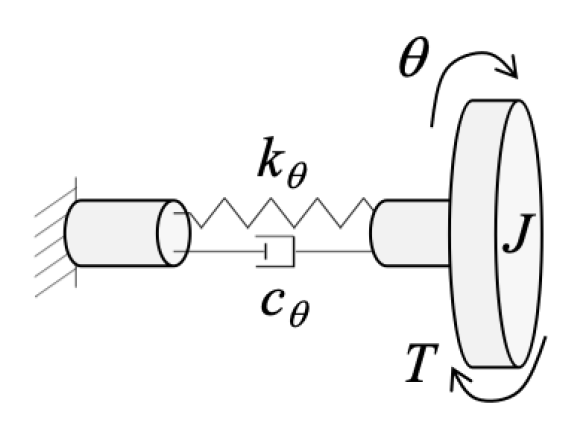
\includegraphics[width=6cm]{images/Q3.png}
\end{figure}

\subsection{a)}
Find the state space representation of this system.
\subsubsection{\textit{ Sol. }}

Define the state vector: $\textbf{x} = 
\begin{bmatrix}
    x_1\\
    x_2
\end{bmatrix} = 
\begin{bmatrix}
    \theta\\
    \dot{\theta}
\end{bmatrix}$, input $u = T$, and output $y = \theta$.

We can write the equation of motion as: $J\ddot{\theta} = - k_{\theta}\theta - c_{\theta}\dot{\theta} + T$ $\Rightarrow $   $\ddot{\theta} = - \frac{k_{\theta}}{J}\theta - \frac{c_{\theta}}{J}\dot{\theta} + \frac{1}{J}T$

\begin{equation} \label{eq:9}
    \begin{aligned} 
        \dot{\textbf{x}} &= 
        \begin{bmatrix}
            0 & 1 \\
            -\frac{k_{\theta}}{J} & -\frac{c_{\theta}}{J}
        \end{bmatrix}
        \textbf{x} + 
        \begin{bmatrix}
            0\\
            \frac{1}{J}
        \end{bmatrix}
        u
        \\
        y &=
        \begin{bmatrix}
            1 & 0
        \end{bmatrix}
        \textbf{x} + 
        \begin{bmatrix}
            0
        \end{bmatrix}
        u
    \end{aligned}
\end{equation}



\subsection{b)}
Now assume that your input torque $T$ is a function of the system state so that
$T = R - \textbf{k}\textbf{x}$ where $\textbf{k}$ is a vector $\begin{bmatrix}k_1 & k_2\end{bmatrix}$ and $\textbf{x}$ is the state vector. Find the new state equation assuming a new input, $u = R$.

\subsubsection{\textit{ Sol. }}

Substitute $u$ in Eq.\ref{eq:9} with 
$\left(R - \begin{bmatrix} k_1 & k_2 \end{bmatrix} \textbf{x}\right)$ we get:

\begin{equation}
    \begin{split}
        \dot{\textbf{x}} &= 
        \begin{bmatrix}
            0 & 1 \\
            -\frac{k_{\theta}}{J} & -\frac{c_{\theta}}{J}
        \end{bmatrix}
        \textbf{x} + 
        \begin{bmatrix}
            0\\
            \frac{1}{J}
        \end{bmatrix}
        \left(R - \begin{bmatrix} k_1 & k_2 \end{bmatrix}
        \textbf{x}
        \right) \\
        &= 
        \left(\begin{bmatrix}
            0 & 1 \\
            -\frac{k_{\theta}}{J} & -\frac{c_{\theta}}{J}
        \end{bmatrix} - \begin{bmatrix}
            0\\
            \frac{1}{J}
        \end{bmatrix}\begin{bmatrix}
            k_1 & k_2
        \end{bmatrix}\right)
        \textbf{x} + 
        \begin{bmatrix}
            0\\
            \frac{1}{J}
        \end{bmatrix}R
        \\
        &= 
        \begin{bmatrix}
            0 & 1 \\
            -\frac{k_{\theta} + k_1}{J}& -\frac{c_{\theta} +k_2}{J}
        \end{bmatrix}
        \textbf{x} + 
        \begin{bmatrix}
            0\\
            \frac{1}{J}
        \end{bmatrix}R\\
        &= 
        \begin{bmatrix}
            0 & 1 \\
            -\frac{k_{\theta} + k_1}{J}& -\frac{c_{\theta} +k_2}{J}
        \end{bmatrix}
        \textbf{x} + 
        \begin{bmatrix}
            0\\
            \frac{1}{J}
        \end{bmatrix}u\\ 
        y &=
        \begin{bmatrix}
            1 & 0
        \end{bmatrix}
        \textbf{x} + 
        \begin{bmatrix}
            0
        \end{bmatrix}
        \left(R - \begin{bmatrix} k_1 & k_2 \end{bmatrix}
        \textbf{x}
        \right) \\
        &= \begin{bmatrix}
            1 & 0
        \end{bmatrix}
        \textbf{x} + 
        \begin{bmatrix}
            0
        \end{bmatrix}u
    \end{split}
\end{equation}

\subsection{c)}
Assuming $J = 1\ kg\cdot m^2$, $c_{\theta} =2\ N\cdot m\cdot s/rad$, $k_{\theta} =5\ N\cdot m/rad$, simulate the response to a step input of $0.1\ N\cdot m$ for the original system and a step of $0.64\ N\cdot m$ for the new system with $k =\begin{bmatrix}27 & 6\end{bmatrix}$.

\subsubsection{\textit{ Sol. }}
Matlab code:
\lstinputlisting{codes/Question3c.m}
Result:
\begin{figure}[htp]
    \centering
    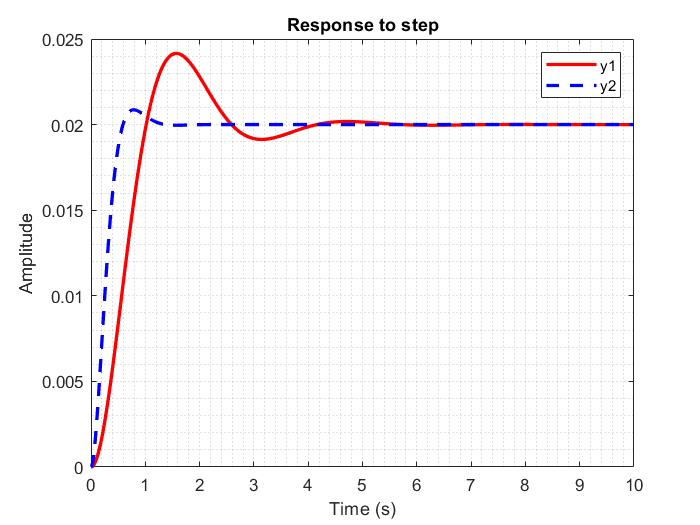
\includegraphics[width=15cm]{images/Q3_c_fig.png}
    \caption{Step Response}
    \label{fig:Q3c}
\end{figure}
\pagebreak
    \section{Problem 4}
State space representation with input derivatives.

For the following mechanical system, input is the displacement $u$ and output is the displacement $z$.

\begin{figure}[htp]
    \centering
    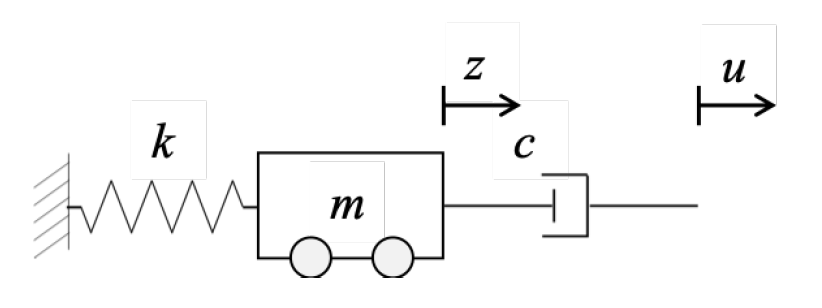
\includegraphics[width=6cm]{images/Q4.png}
\end{figure}

\subsection{a)}
Find the state space representation of this system.
\subsubsection{\textit{ Sol. }}

Draw FBD to analyze system dynamics: 
\begin{figure}[htp]
    \centering
    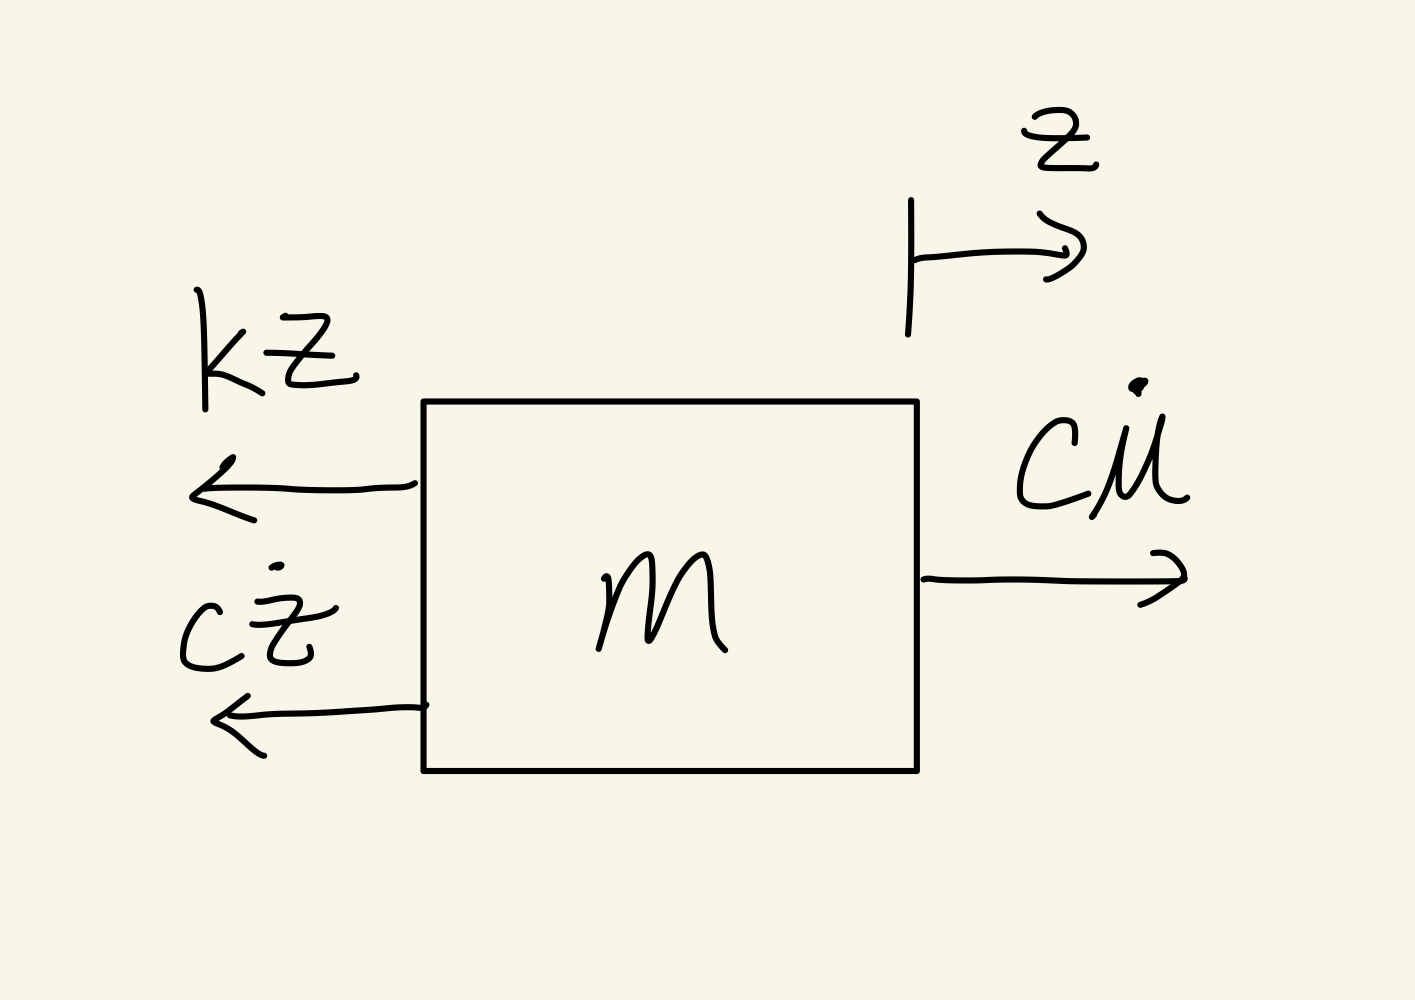
\includegraphics[width=6cm]{images/Q4_FBD.png}
    \caption{Free body diagram}
    \label{fig:Q4FBD}
\end{figure}

We get the following dynamic equation: $m\ddot{z} = -kz-c\dot{z}+c\dot{u}$ $\Rightarrow$ $\ddot{z} = -\frac{k}{m}z-\frac{c}{m}\dot{z}+\frac{c}{m}\dot{u}$

Because we have derivative of input, we can define the state vector as: $\textbf{x} = 
\begin{bmatrix}
    x_1\\
    x_2
\end{bmatrix} = 
\begin{bmatrix}
    z\\
    \dot{z} - \frac{c}{m}u
\end{bmatrix}$, and output $y = z$.

From $\ddot{z} = -\frac{k}{m}z-\frac{c}{m}\dot{z}+\frac{c}{m}\dot{u}$ 

$\Rightarrow$     
$\left\{
    \begin{array}{lr}
    \dot{x_1} = \dot{z} = \left(\dot{z} - \frac{c}{m}u\right) +  \frac{c}{m}u = x_2 + \frac{c}{m}u\\
    \dot{x_2} = \ddot{z} - \frac{c}{m}\dot{u} = -\frac{k}{m}z-\frac{c}{m}\dot{z}+\frac{c}{m}\dot{u} - \frac{c}{m}\dot{u} = -\frac{k}{m}z - \frac{c}{m}(x_2 + \frac{c}{m}u) = -\frac{k}{m}x_1 - \frac{c}{m}x_2 - \left(\frac{c}{m}\right)^2u
    \end{array}
\right.$ 

We get: 
\begin{equation}
    \begin{aligned}
        \dot{\textbf{x}} &=
        \begin{bmatrix}
            0 & 1 \\
            -\frac{k}{m} & -\frac{c}{m}
        \end{bmatrix}
        \textbf{x} + 
        \begin{bmatrix}
            \frac{c}{m}\\
            -\left(\frac{c}{m}\right)^2
        \end{bmatrix}
        u
        \\
        y &=
        \begin{bmatrix}
            1 & 0
        \end{bmatrix}
        \textbf{x} + 
        \begin{bmatrix}
            0
        \end{bmatrix}
        u
    \end{aligned}
\end{equation}
\subsection{b)}
Assume that $m =10 kg$, $c =20 N-s/m$, $k =40 N/m$, and the input displacement is a step displacement of $0.2 m$. Use Matlab to plot the response $z(t)$. Include your code and plot. Is there anything unusual about this step response? Why is this the case for this system?

Matlab code:
    \lstinputlisting{codes/Question4b.m}
Result:
\begin{figure}[htp]
    \centering
    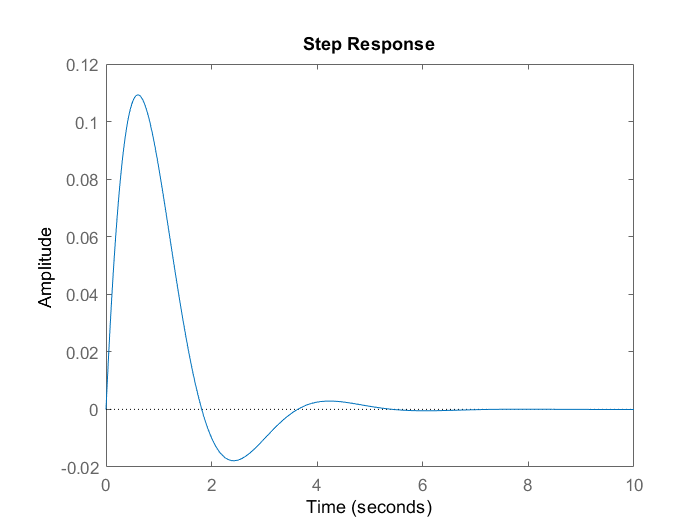
\includegraphics[width=12cm]{images/Q4_b_fig.png}
    \caption{Step Response}
    \label{fig:Q4b}
\end{figure}

The step response is as expected. The final value goes to zero, because the first derivative of the input $u$ only changes at time $0_{+}$, thus energy is added to the system only at time $0_{+}$. And because this is a damped system, total energy in the system will eventually dissipate to zero.
\pagebreak
    \section{Problem 5}
Transfer function to state space.

For each of the transfer functions shown, write the corresponding differential equation and provide a state space representation.
\subsection{a)}
\begin{equation}
    \frac{\Theta_1(s)}{T_1(s)} = \frac{100}{s^4+20s^3+10s^2+7s+100}
\end{equation}
\subsubsection{\textit{ Sol. }}
Convert the given transfer function to standard format:
$\frac{\Theta_1(s)}{T_1(s)} = \frac{b_1s^3+b_2s^2+b_3s+b_4}{s^4+a_1s^3+a_2s^2+a_3s+a_4}$, 

where $b_1 = b_2=b_3=0$, $b_4 = 100$, $a_1 = 20$, $a_2 = 10$, $a_3 = 7$, $a_4 = 100$.

We have:
\begin{equation}
    \begin{aligned}
        \dot{\textbf{x}} &=
        \begin{bmatrix}
            0    & 1    & 0    & 0\\
            0    & 0    & 1    & 0\\
            0    & 0    & 0    & 1\\
            -a_4 & -a_3 & -a_2 & -a_1
        \end{bmatrix}
        \textbf{x} + 
        \begin{bmatrix}
            0 \\ 0 \\ 0 \\ 1
        \end{bmatrix}
        u \\ &=
        \begin{bmatrix}
            0    & 1    & 0    & 0\\
            0    & 0    & 1    & 0\\
            0    & 0    & 0    & 1\\
            -100 & -7   & -10  & -20
        \end{bmatrix}
        \textbf{x} + 
        \begin{bmatrix}
            0 \\ 0 \\ 0 \\ 1
        \end{bmatrix}
        u \\
        \dot{\textbf{y}} &=
        \begin{bmatrix}
            b_4 & b_3 & b_2 & b_1
        \end{bmatrix}
        \textbf{x} + 
        \begin{bmatrix}
            0
        \end{bmatrix}
        u \\ &=
        \begin{bmatrix}
            100 & 0 & 0 & 0
        \end{bmatrix}
        \textbf{x} + 
        \begin{bmatrix}
            0
        \end{bmatrix}
        u
    \end{aligned}
\end{equation}

Matlab code:
    \lstinputlisting{codes/Question5a.m}
Result:
\begin{figure}[htp]
    \centering
    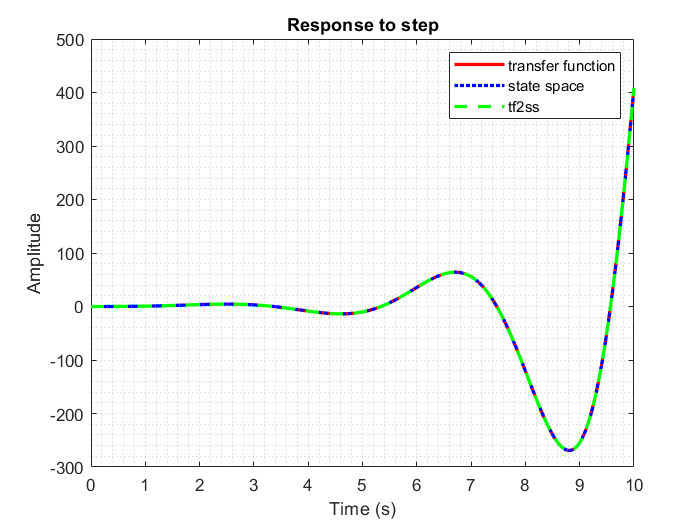
\includegraphics[width=12cm]{images/Q5_a_fig.png}
    \caption{Step Response}
    \label{fig:Q5a1}
\end{figure}


\subsection{b)}
\begin{equation}
    \frac{Y_1(s)}{F_1(s)} = \frac{8s+10}{s^3+s^2+5s+13}
\end{equation}

\subsubsection{\textit{ Sol. }}
Convert the given transfer function to standard format:
$\frac{Y_1(s)}{F_1(s)} = \frac{b_1s^2+b_2s+b_3}{s^3+a_1s^2+a_2s+a_3}$, 

where $b_1 =0$, $b_2=8$, $b_3 = 10$, $a_1 = 1$, $a_2 = 5$, $a_3 = 13$.

We have:
\begin{equation}
    \begin{aligned}
        \dot{\textbf{x}} &=
        \begin{bmatrix}
            0    & 1    & 0\\
            0    & 0    & 1\\
            -a_3 & -a_2 & -a_1
        \end{bmatrix}
        \textbf{x} + 
        \begin{bmatrix}
            0 \\ 0 \\ 1
        \end{bmatrix}
        u \\ &=
        \begin{bmatrix}
            0    & 1    & 0\\
            0    & 0    & 1\\
            -13  & -5   & -1
        \end{bmatrix}
        \textbf{x} + 
        \begin{bmatrix}
            0 \\ 0 \\ 1
        \end{bmatrix}
        u \\
        \dot{\textbf{y}} &=
        \begin{bmatrix}
            b_3 & b_2 & b_1
        \end{bmatrix}
        \textbf{x} + 
        \begin{bmatrix}
            0
        \end{bmatrix}
        u \\ &=
        \begin{bmatrix}
            10 & 8 & 0
        \end{bmatrix}
        \textbf{x} + 
        \begin{bmatrix}
            0
        \end{bmatrix}
        u
    \end{aligned}
\end{equation}

Matlab code:
    \lstinputlisting{codes/Question5b.m}
Result:
\begin{figure}[htp]
    \centering
    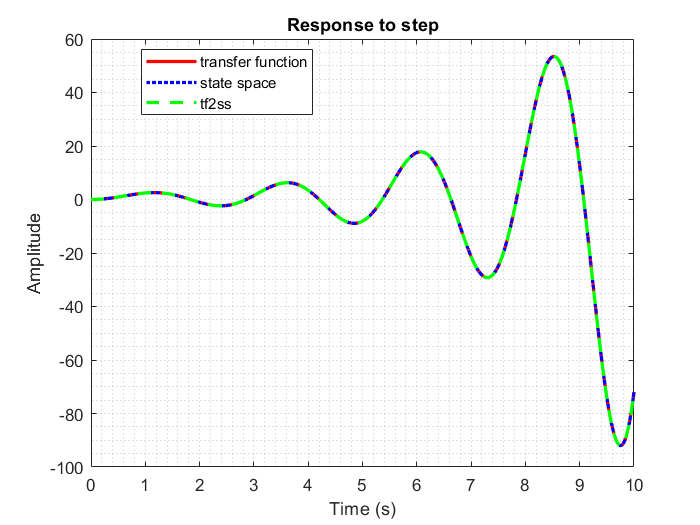
\includegraphics[width=12cm]{images/Q5_b_fig.png}
    \caption{Step Response}
    \label{fig:Q5a1}
\end{figure}
\pagebreak
    \section{Problem 6}
State space to transfer function.

In general, state space representations are not unique as discussed in lecture. You are given the following systems.


    \begin{align}
        \begin{bmatrix}
            \dot{x} \\
            \ddot{x}
        \end{bmatrix} &=
        \begin{bmatrix}
            -5 & 0 \\
            0  & -1
        \end{bmatrix}
        \begin{bmatrix}
            x \\
            \dot{x}
        \end{bmatrix} + 
        \begin{bmatrix}
            3\\
            1
        \end{bmatrix}
        u \label{eq:16}
        \\
        y &=
        \begin{bmatrix}
            7 & 0
        \end{bmatrix}
        \begin{bmatrix}
            x \\
            \dot{x}
        \end{bmatrix} \label{eq:17}
    \end{align}



\begin{align}
    \begin{bmatrix}
        \dot{x} \\
        \ddot{x}
    \end{bmatrix} &=
    \begin{bmatrix}
        -5 & 0 \\
        0  & -1
    \end{bmatrix}
    \begin{bmatrix}
        x \\
        \dot{x}
    \end{bmatrix} + 
    \begin{bmatrix}
        3\\
        0
    \end{bmatrix}
    u\label{eq:18}
    \\
    y &=
    \begin{bmatrix}
        7 & 3
    \end{bmatrix}
    \begin{bmatrix}
        x \\
        \dot{x}
    \end{bmatrix}\label{eq:19}
\end{align}

\subsection{a)}
Analytically (by hand!) show that these systems will result in the same transfer
function $\frac{Y(s)}{U(s)}$.
\subsubsection{\textit{ Sol. }}

Start by doing Laplace transform on state equation in Eq.\ref{eq:16} and Eq.\ref{eq:17}:

\begin{align}
    \mathcal{L} \{\dot{\textbf{x}}\} &= sX(s) = AX(s) + BU(s) \label{eq:20}\\ 
    \mathcal{L} \{y\} &= Y(s) = CX(s) + DU(s) \label{eq:21}
\end{align}
From Eq.\ref{eq:20} we get:
\begin{equation}
    X(s) = (sI - A)^{-1}BU(s) \label{eq:22}
\end{equation}

Replace $X(s)$ in Eq.\ref{eq:21} with Eq.\ref{eq:22}
\begin{equation}
    Y(s) = (C(sI - A)^{-1}B + D)U(s) \label{eq:23}
\end{equation}
So we have: 
\begin{equation}
    \begin{aligned}
        \frac{Y(s)}{U(s)} &= C(sI - A)^{-1}B + D \\
        &= \begin{bmatrix} 7 & 0 \end{bmatrix}
        (\begin{bmatrix} s & 0 \\ 0 & s \end{bmatrix} -
        \begin{bmatrix} -5 & 0 \\ 0 & -1 \end{bmatrix})^{-1}
        \begin{bmatrix} 3\\1\end{bmatrix} + 0 \\ 
        &= \begin{bmatrix} 7 & 0 \end{bmatrix}\left(\frac{1}{(s+1)(s+5)}\begin{bmatrix}
            s+1 & 0 \\
            0   & s+5
        \end{bmatrix}\right)\begin{bmatrix} 3\\1\end{bmatrix}\\ 
        &= \begin{bmatrix} 7 & 0 \end{bmatrix}\begin{bmatrix} \frac{3}{(s+5)} \\ \frac{1}{(s+1)} \end{bmatrix}\\ 
        &=\frac{21}{s+5}
    \end{aligned}
\end{equation}

Now we do the same to Eq.\ref{eq:18} and Eq.\ref{eq:19}:
\begin{equation}
    \begin{aligned}
        \frac{Y(s)}{U(s)} &= C(sI - A)^{-1}B + D \\
        &= \begin{bmatrix} 7 & 3 \end{bmatrix}
        (\begin{bmatrix} s & 0 \\ 0 & s \end{bmatrix} -
        \begin{bmatrix} -5 & 0 \\ 0 & -1 \end{bmatrix})^{-1}
        \begin{bmatrix} 3\\0\end{bmatrix} + 0 \\ 
        &= \begin{bmatrix} 7 & 3 \end{bmatrix}\left(\frac{1}{(s+1)(s+5)}\begin{bmatrix}
            s+1 & 0 \\
            0   & s+5
        \end{bmatrix}\right)\begin{bmatrix} 3\\0\end{bmatrix}\\ 
        &= \begin{bmatrix} 7 & 3 \end{bmatrix}\begin{bmatrix} \frac{3}{(s+5)} \\ 0 \end{bmatrix}\\ 
        &=\frac{21}{s+5}
    \end{aligned}
\end{equation}

We get the same transfer function $\frac{Y(s)}{U(s)} = \frac{21}{s+5}$.

\subsection{b)}
Matlab code:
    \lstinputlisting{codes/Question6b.m}
Result:
\begin{figure}[htp]
    \centering
    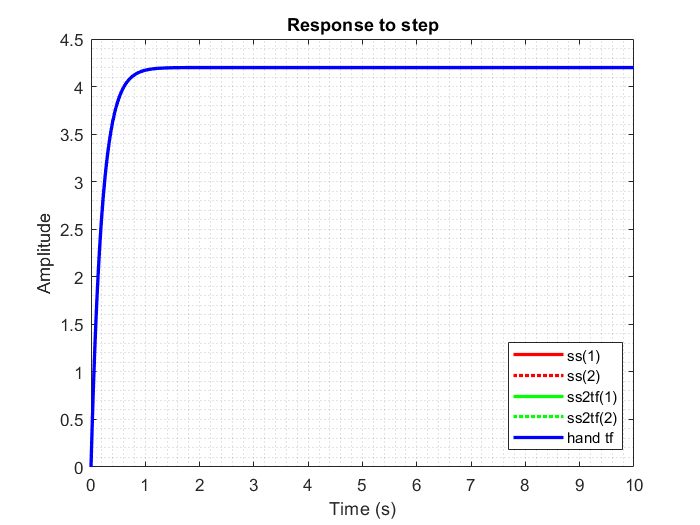
\includegraphics[width=12cm]{images/Q6_b_fig.png}
    \caption{Step Response}
    \label{fig:Q6b}
\end{figure}
\pagebreak
    % 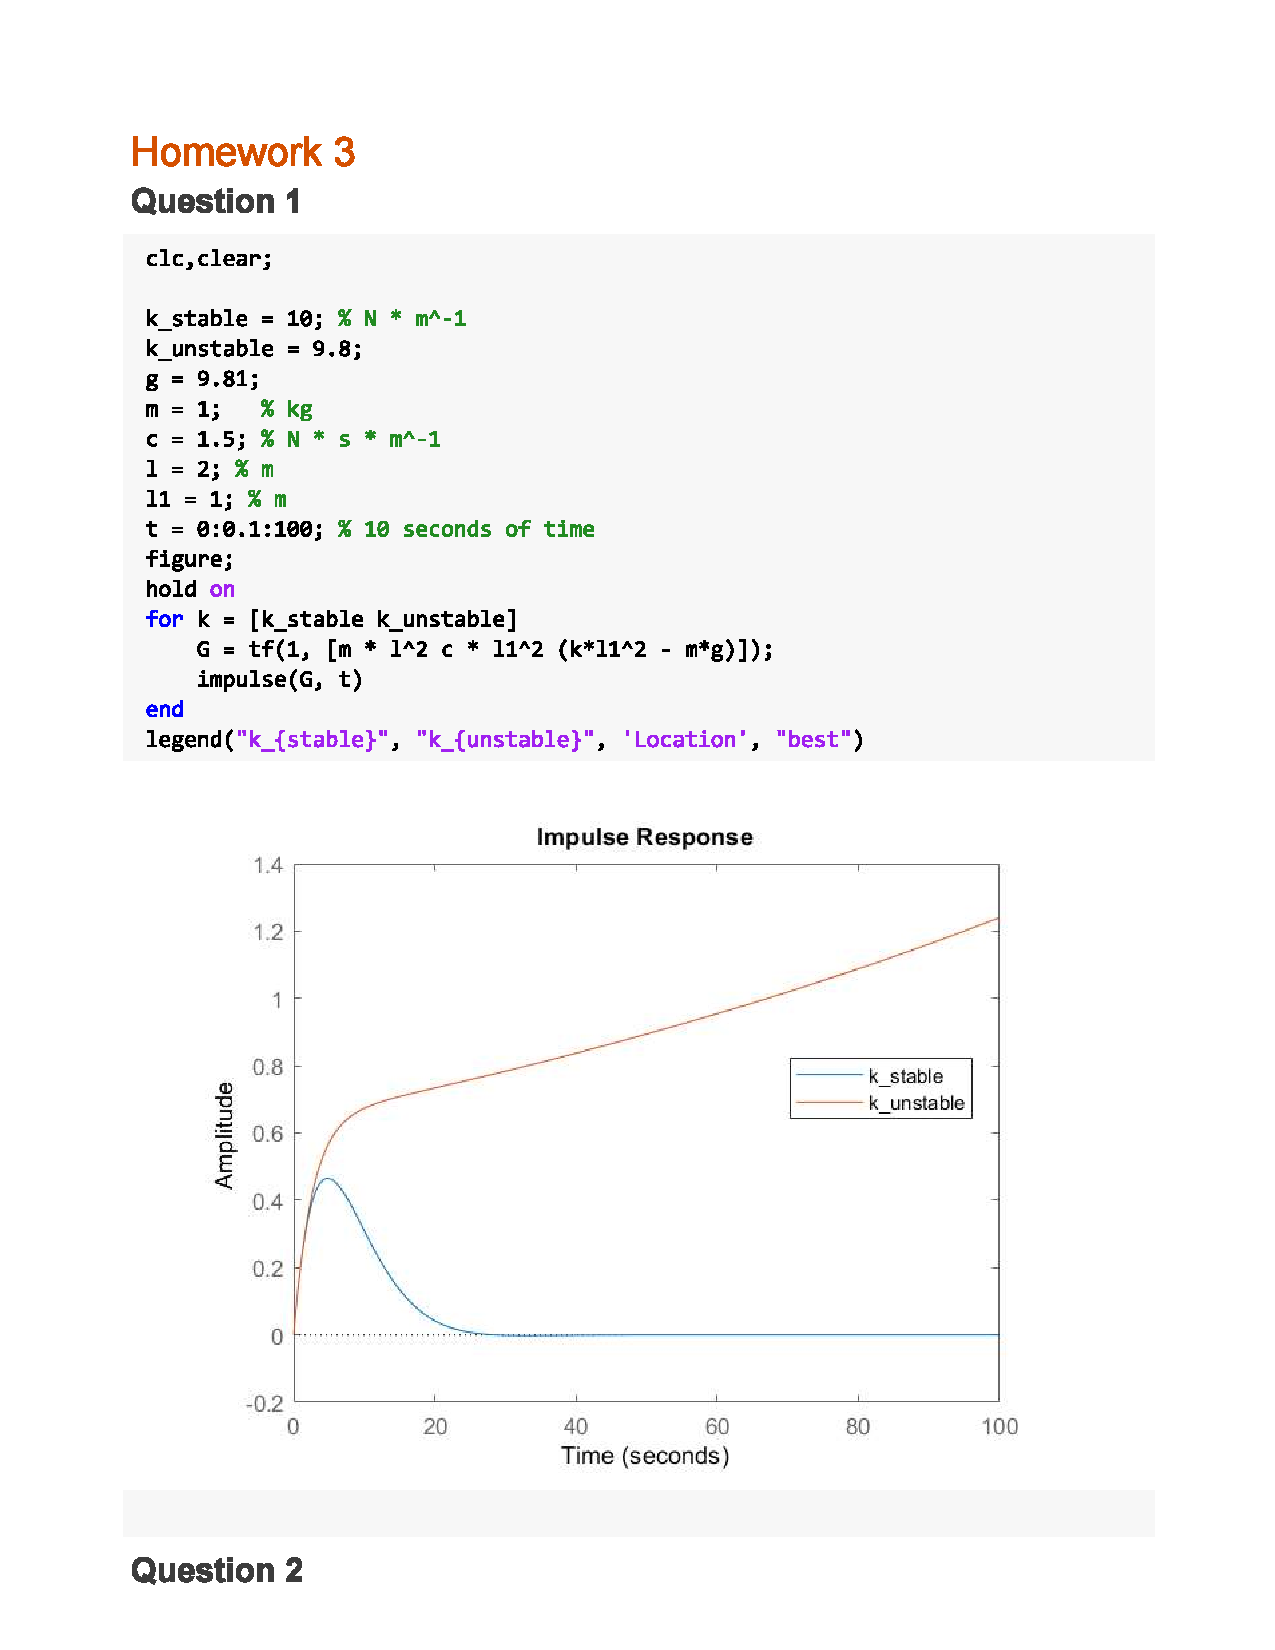
\includepdf{misc/matlab_p1.pdf}
    % % Print the bibliography!
\printbibliography

\end{document}
